% 南京大奸杀
% 南京大奸杀.tex

\documentclass[12pt,UTF8]{ctexbook}

% 设置纸张信息。
\usepackage[a4paper,twoside]{geometry}
\geometry{
	left=25mm,
	right=25mm,
	bottom=25.4mm,
	bindingoffset=10mm
}

% 设置字体,并解决显示难检字问题。
\xeCJKsetup{AutoFallBack=true}
\setCJKmainfont{SimSun}[BoldFont=SimHei, ItalicFont=KaiTi, FallBack=SimSun-ExtB]

% 目录 chapter 级别加点(.)。
\usepackage{titletoc}
\titlecontents{chapter}[0pt]{\vspace{3mm}\bf\addvspace{2pt}\filright}{\contentspush{\thecontentslabel\hspace{0.8em}}}{}{\titlerule*[8pt]{.}\contentspage}

% 设置 part 和 chapter 标题格式。
\ctexset{
	chapter/name={},
	chapter/number={},
	section/name={},
	section/number={},
	subsection/name={},
	subsection/number={}
}

% 图片相关设置。
\usepackage{float}
\usepackage{graphicx}
\graphicspath{{Images/}}

% 设置署名格式。
\newenvironment{shuming}{\hfill\zihao{4}}

% 注脚每页重新编号,避免编号过大。
\usepackage[perpage]{footmisc}

\title{\heiti\zihao{0} 南京大奸杀}
\author{素丹}
\date{}

\begin{document}

\maketitle
\tableofcontents

\frontmatter

\begin{figure}[htbp]
	\centering
	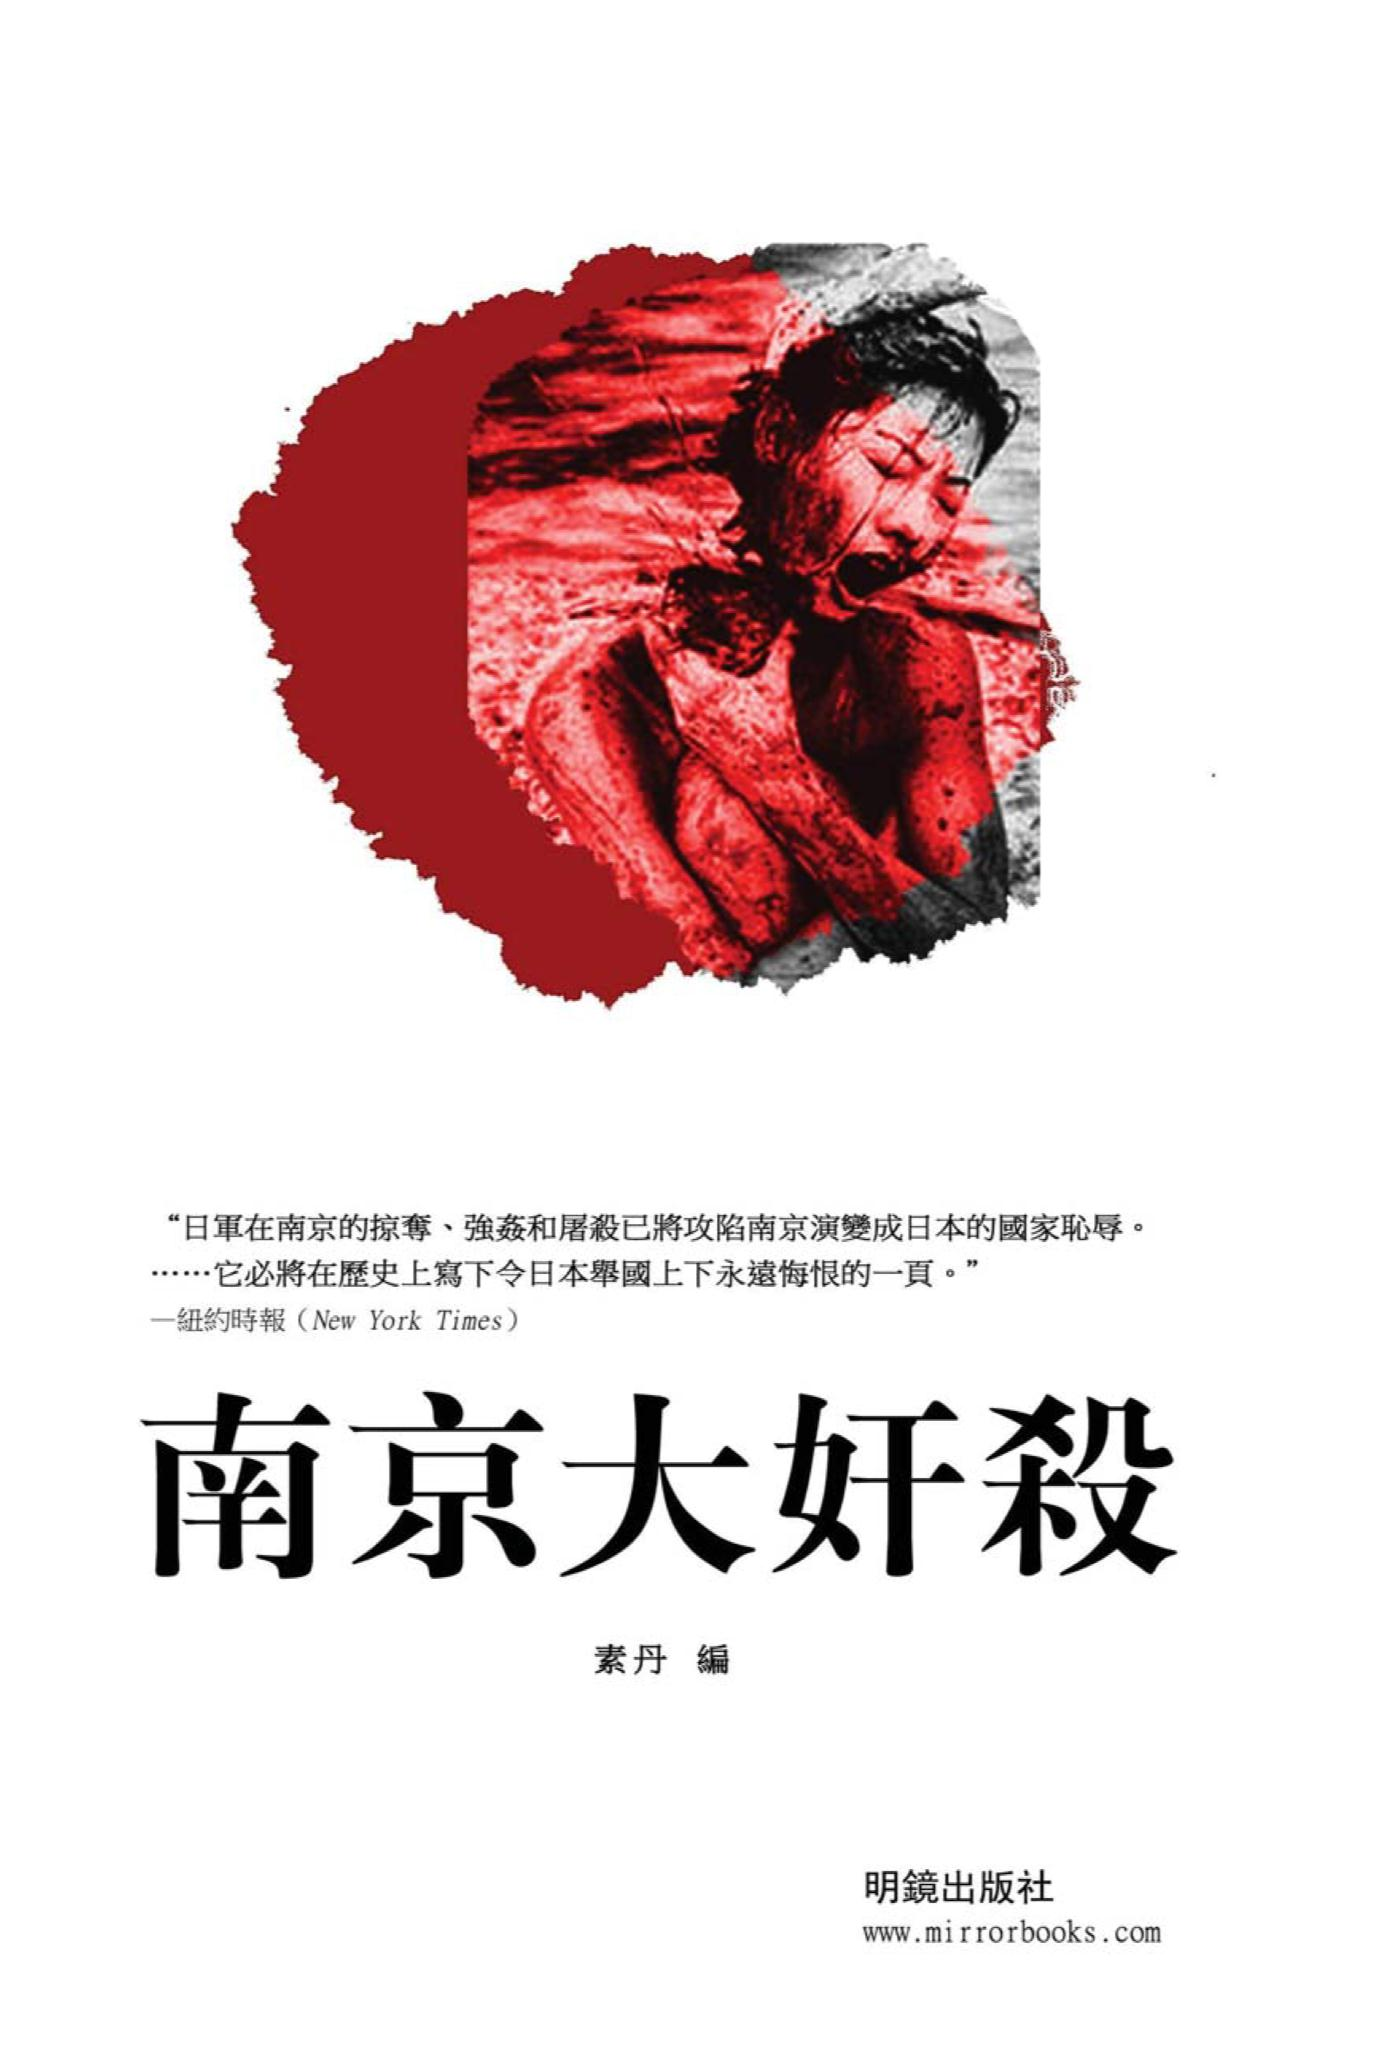
\includegraphics[width=0.7\linewidth]{cover}
	\caption{}
	\label{fig:1}
\end{figure}

\begin{figure}[htbp]
	\centering
	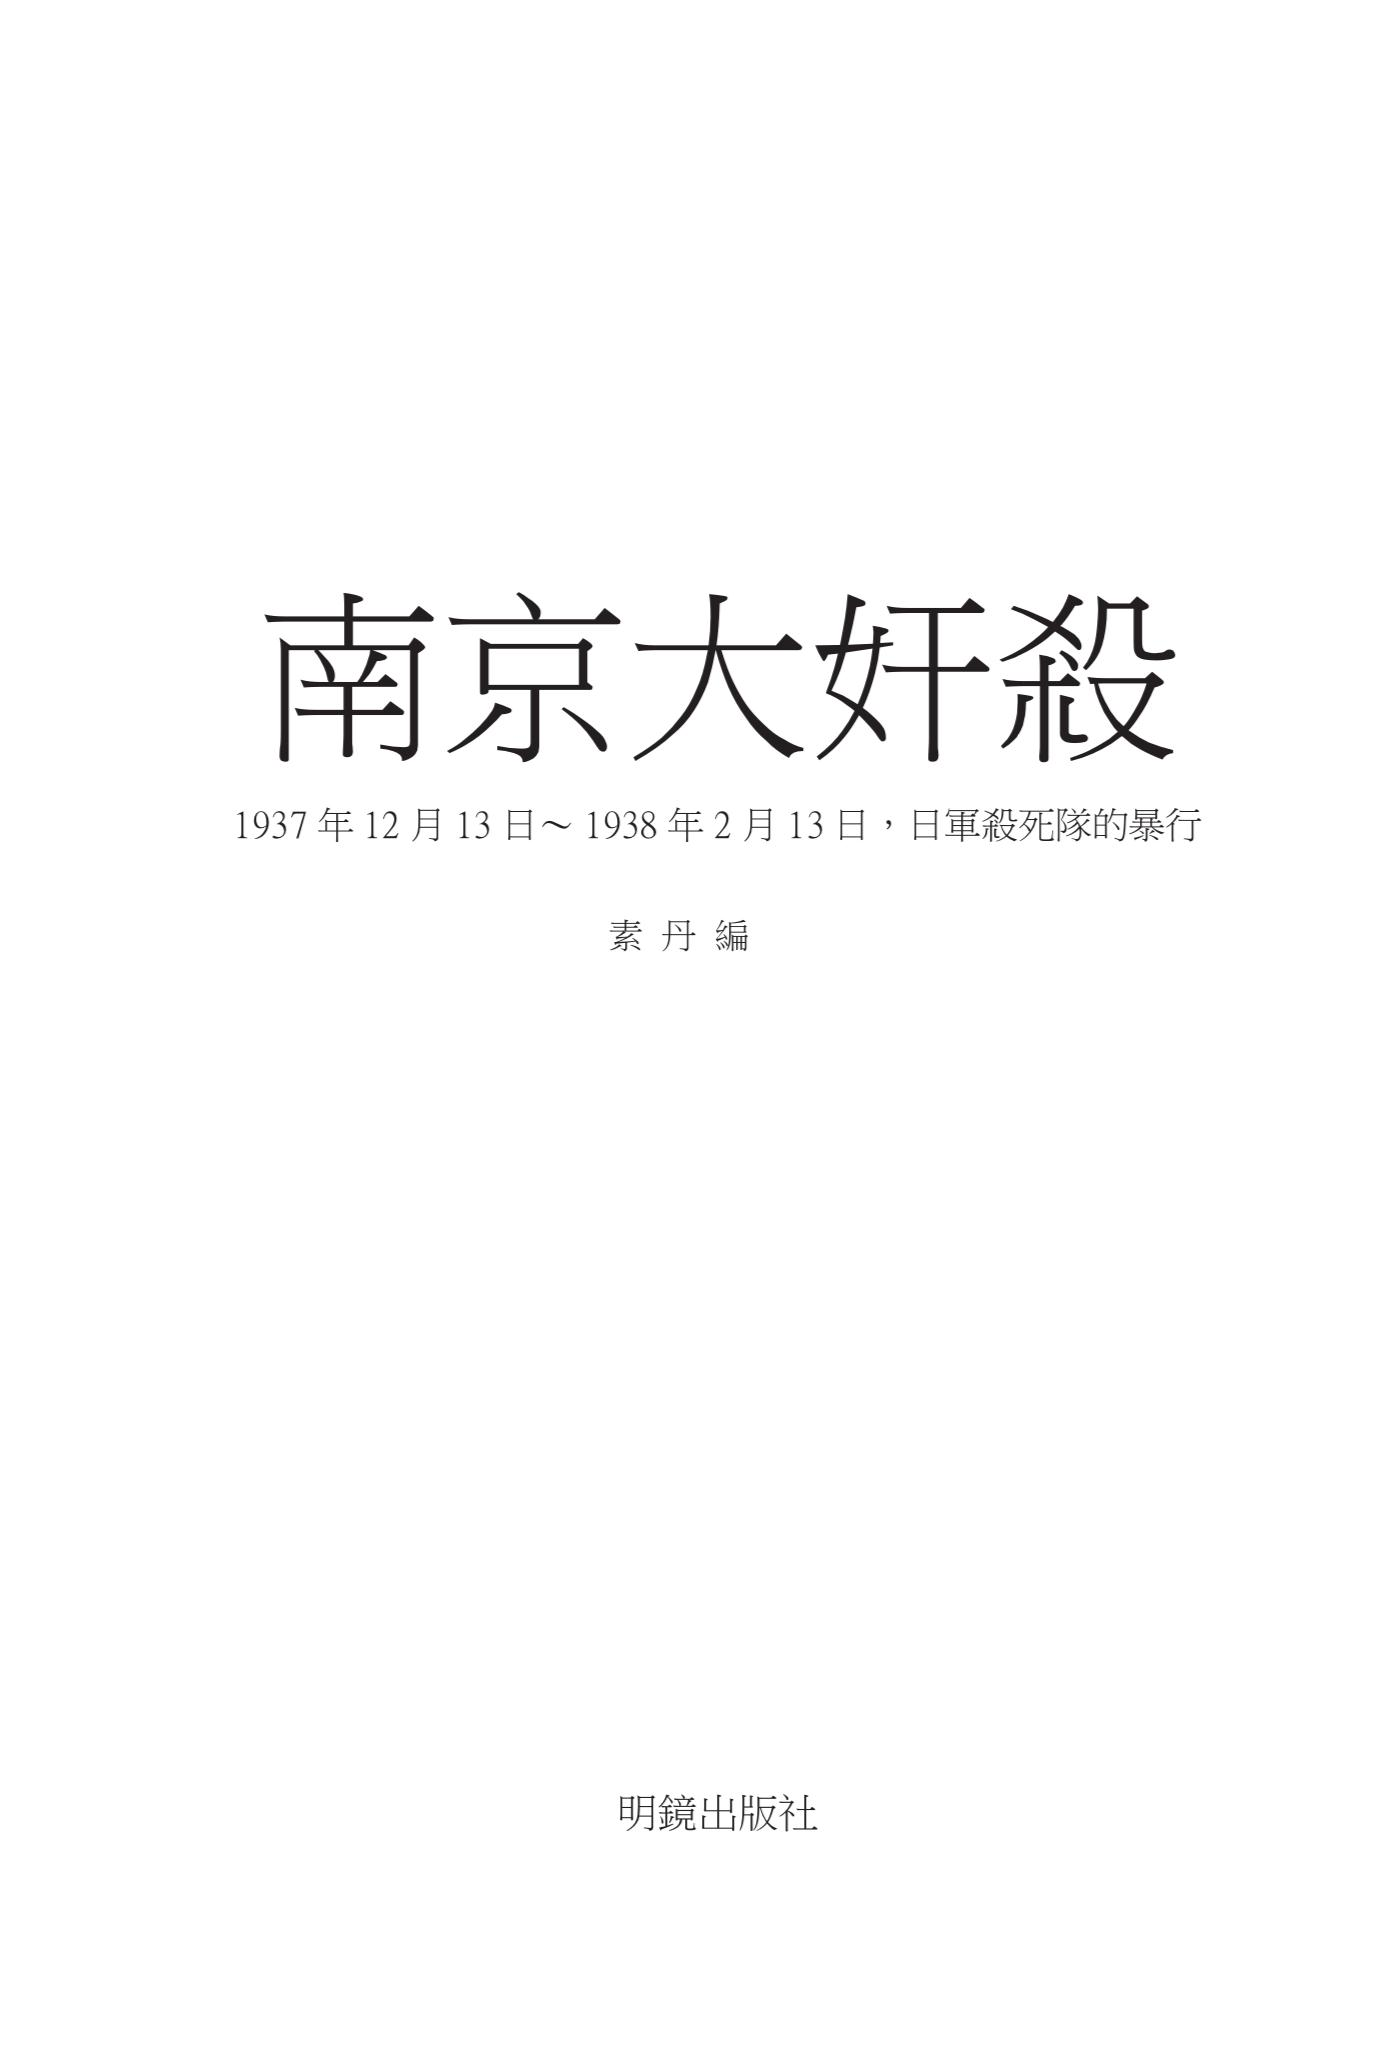
\includegraphics[width=0.7\linewidth]{cover1}
	\caption{}
	\label{fig:1}
\end{figure}

\begin{figure}[htbp]
	\centering
	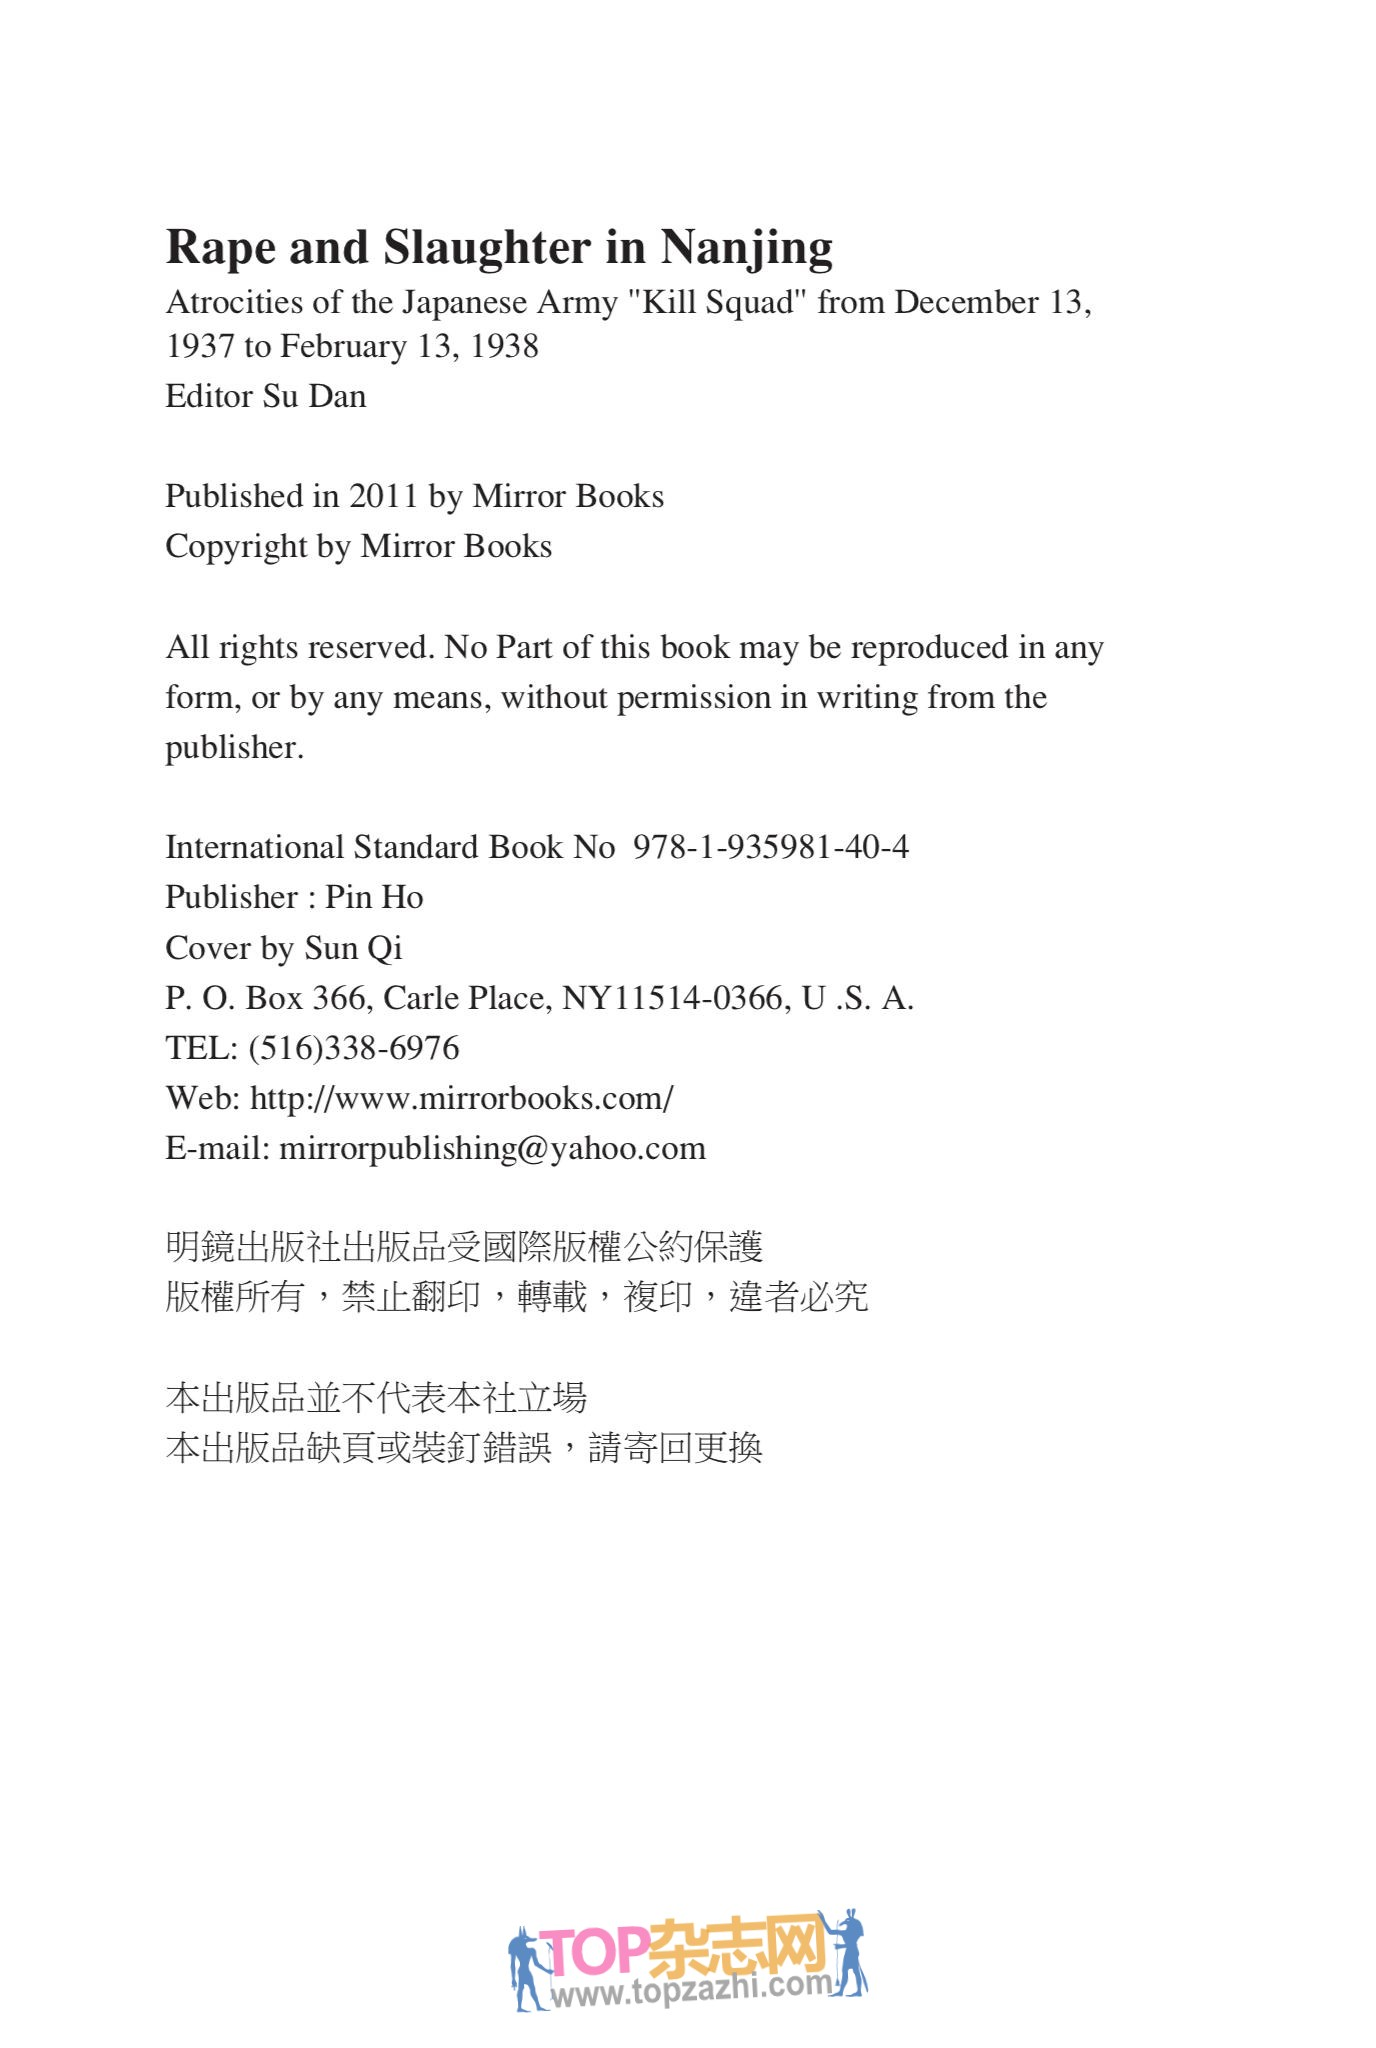
\includegraphics[width=0.7\linewidth]{cover2}
	\caption{}
	\label{fig:1}
\end{figure}

“跟女人干时,她们是人;等你宰她们时,她们就是猪了。”
——(日兵)东史郎《罪孽的报应》,Ian Buruma著,社会科学文献出版社,2006年版

魔鬼分队长

山口宰太郎官拜下士,隸屬陸軍步兵第一二四連隊,骠悍善戰,戰
功彪炳,人人尊稱“魔鬼分隊長”,曾獲天皇賜頒勋章。

魔鬼分隊長身經百戰,唯一的一次受傷是在西伯利亞戰線,當時七
個兵團的兵力被梅毒消滅掉一個兵團,多亏盤尼西林,他侥幸死裹
逃生,得以派赴中國戰場。當大军從登陸杭州灣到攻估南京,神勇
的魔鬼分隊長,以每天最少强奸四個妇女的戰绩領先袍澤。

魔鬼分隊長,天赋異禀,每毫升精液含有兩萬五千九百九十九隻凶
猛的精蟲,每次射精量約二十C·C·,每月可生產十七加侖腐蚀性极強
的新鲜精液。每逢月圆,會出現三個睾九,那根金属般的陰萃長
度則增加十三公分。

魔鬼分隊長忠心耿耿,每次性交前都要先立正唱國歌。

焦桐《世纪詩選》(臺灣),2000:98 ~ 99

\chapter{野兽的战争(代前言)}

\section{1}

“中國人皆可殺。” 日軍第 16 師團師
團長、陸軍中将中島今朝吾說。而他的
首長上海派遣軍司令官、陸軍中將朝香
宮鳩彥(あさかのみややすひこおう,昭和天皇裕仁的
叔父、南京大屠毅的策劃和發動者)則在1937年12
月5日下違的一
份由他簽名蓋章且標明“機密,阅後銷毁”的字樣的命令,内容只有六個字:“全部杀掉俘虏。”

“……強盗式的掠奪和强奸,為士氣
旺盛之所寄。”日軍第6師團師團長、陸
軍中將谷壽夫在撰寫的《陸戰術》中說。
而他的首長第 10 軍司令官、陸軍中將柳
川平助則在演講中說:“(中國)山川草木皆是敵人。”

上海派遣军和第 10 军是日本大本营(天皇直屬的陸海軍最高统帥機構)命令组建的华中
方面軍的兩個戰鬥序列。華中方面军的最高司令官是松井石根大將。松井大将
則在攻陷南京後下達屠杀戰俘、平民(括婦女、兒童和老人)的命令:“纪律肅正。”

攻占南京,30萬中國軍民毫無尊嚴
地死去。這是日本欲消滅中國,實現稱
霸世界的野心中的第一屠宰場。而這将
使整個人類蒙羞。

\section{2}

1931年9月18日,日軍炸毁滿铁
線路栽贓中國軍而突襲且占领东北三
省;1937年7月7日,在北京卢沟桥发
生的一名日兵失蹤事件成為日軍預謀揮
動屠刀、侵占全中國的藉口。攻城掠地。
一個城市接著一個城市,一個乡村接著
一個鄉村渝陷。重要的城市天津、北京
和上海先後沦陷。日本盯上了距離上海
400公里的南京--蒋介石的中華民國
政府的首都。欲讓蒋“投降”,必先傾覆
他的巢穴。

松井大将在1937年12月1日接到
日本大本營的指令:“攻占敵國首都南
京。”从杭州灣登陸的第 10 军和上海派
遣军,超過 20萬軍隊,兵分三路,成包
圍熊勢向南京急行軍。

\section{3}

為了攫取戰功,日軍日夜奔襲,“一
刻也得不到休息”,“一邊打著瞌睡,一
邊行進”;軍方下達命令:“糧草在當地
徵發,自謀活路。”“将被服、糧食放在
途中的兵站基地,僅带著武器彈藥前進。
士兵接替軍馬拖拉貨车。”日重聲稱後勤
的物資保障皆由“蒋介石提供”。

但提供糧草的只能是無辜的城乡居
民。日軍不但掠奪糧草,还實行“四光”(杀
光、燒光、搶光、女人奸光)政策。第10軍第6
師團司令部接到命令“不管女人還是孩
子,只要是支那人就统统殺掉,房屋全
部燒掉!”

一個任大隊長一職的少佐鼓勵手下
的日兵說:“要讓蒋介石投降,僅僅攻陷
南京是不夠的,要用一切手段讓清國奴
們陷入恐怖。看見清國奴就殺死他們,
即使是百姓。還可以掠奪,强奸女性也
行,放火也可以。”

一名日兵告訴他的戰友說,上司下
达命令,“一旦發現清國奴,不管他是
士兵還是百姓,見一個殺一個。只要看
到女人,不管是姑娘還是已為人妻,全
都强奸,而且完事之後肯定殺死。”

天皇的軍隊所到之處,像蝗蟲經過。
糧食抢光,房屋燒光。男人和幼童殺死。
女人輪奸後殺死;日軍嫌槍殺和刺死中
國士兵麻煩,甚至把戰俘驱逐到路當中
讓行進中的坦克戰車碾死。

日军上海派遣军第16師團輜重兵
一名一等兵,後來在他的从軍回忆錄中
寫道:“馬路邊有用磚圍起來的墳墓。
所到之處,士兵們都會把磚拆掉,打開
蓋子進行檢查。如果有中國士兵的屍體,
就脱掉褲子進行檢查。如果是女屍,就
把棍棒插入她的陰部。”

日重第10军第6師團輜重兵一名
小隊長,後來在他撰寫的《不認人的刺
刀》中寫道:沿途放在棺材裹的男人的
屍體被日軍“焚燒”,女人的屍體的“下
腹部都被插上了粗粗的圓木棒”。

一名日兵的話代表了攻佔南京的数
以萬計的日軍的心聲:“到了南京就有
許多漂亮的姑娘……。只想多吃點,培
養好體力。

\section{4}

南京危在旦夕。驚恐萬状的蒋介石,
和他的夫人宋美齡,各乘一架专機在 12
月7日拂曉逃離南京,還先後順带捎走
了南京的軍政官員、戰鬥機、重炮、戰
艦和精銳的軍隊。能動的公共車輛和人
力车都馱著官員逃走了。

獨裁者蒋介石,拒絕西方军事專家
和自己的高級指揮官棄守南京、保存数
十萬生靈的忠告。南京城的背後是長江,
军隊將被困在這兒,“将使城墙内的防禦
變成一場災難”。但蒋寧願以装備很差的
地方部隊表演一場給自己的“遮羞的戲剧”。

“誓與南京共存亡。”中國国民黨南
京衛戍軍司令官、陸軍一級上將唐生智
說。攻擊與防禦,日軍與國軍死傷惨重。
整個南京都被炮彈爆炸的火光照耀得像
蔣介石的臉色一樣惨白。唐上將在 12
月11日的戰鬥中趁夜乘船逃離南京,甚
至连他的指揮部都不知道他的去向。

在南京城,能指望捍衛首都的只剩
下這一群人了:腐朽在中山陵陵墓裹的
革命之父孫中山、超過 10萬名人心崩潰
的守城軍隊、數十萬無辜的平民以及成
千上萬婦女、少女、幼女的贞操。這些
死去的和活著的、被围困的男男女女們
将為身系的國家盡力了。

與此同時,慷慨赴難的還有一群熱
心的人。由15 名外籍人組成的南京難民
安全區國際委員會,和以美籍牧師為主
席的 17人组成的國際紅十字南京委員
會,負起救苦救難的重任,这也是南京
陷落後惟一的行政機構。安全區委員会
主席、納粹德國人拉貝說:“為 20 萬中
國平民提供最後的避難場所。”

12月13日,當日本的太阳旗插上
了中華民國政府高耸的行政樓上後,南
京即告陷落。

松井大將後來在遠東國際軍事法庭
上宣誓說:攻占中國首都南京的行动“不
是出於仇恨而是出於爱”。

\section{5}

日軍屠殺所有能動彈或還喘气的中
國人。南京國民党守城營長郭歧,在首
都渝陷後匿藏難民區,他在撰寫的《陷
都血涙錄》中寫道:“沒有一個男人,敢
說自己活得到明天,没有一個女人,敢
說自己能保得住贞节。”

日軍還把“征服敵人的女性”,“竭
盡全力享受中國女性”,當做“戰果”和
征服者的證據。“令人難於啟齒的野兽行
為”有組織、有預謀地落到了身陷南京
的女人的頭上了。

這一點,甚至连身在南京的德國驻
南京大使館行政主管沙爾芬貝格都瞞不
住了。他在寫给德國外交部的南京局勢
報告中寫道:“日本士兵為什麼能像神
話中的酒鬼戰士一樣兇神惡煞地撲向一
切……我可以肯定地說,就像1918年人
們給黑人的許諾一樣,日本士兵也得到
許諾:只要你們能夠堅持到底,到南京
每人都可以得到一個漂亮的姑娘。”

\section{6}

鐵證如山。血债未償。

此書以加害方——日本政府高級官
員、日本大本營指揮官、日军攻佔南京
的華中方面军将兵、随军記者,與在南
京的中立方——外籍大學教授、医生、
傳教士,駐南京的美國、英國、德國大
使館外交人員、新聞記者,以及在南京
的受害方——女性受害者、中國官兵、
平民,通過政府的絕密檔、戰地日記、
戰鬥詳報丶回憶錄丶觀察日誌丶抗議信
件、秘密外交電文、證人證言等文献史
料,來復原中國女性遭受日军强奸,乃
至輪奸,侮辱活著的或死去的女性阴道
且遭受屠觳後的某個瞬間,審視加害方、
中立方和受害方的所見所聞和内心觸動,
哀悼這場世界文明史和戰爭史上最黑暗、
最殘忍、最邪惡、最悲痛的骇人聽聞的
大屠殺中的大奸殺。

\section{7}

這場已湮沒在時間的長河裹了的反
人類的殺戮,再也無人能完整復原和清
晰記錄,就像無人能撤除日軍犯下的暴行。

但如果對日军在南京杀人如麻以及
強奸、放火、搶劫的暴行進行概括的话,
那将無人能比納粹德國駐南京大使館說
得再精確的了。

納粹德國是日本的戰爭盟友,連它
都不能再容忍這种滅绝人性的暴行了。
它在發給德國外交部的秘密電報中写道:
“犯罪的不是這個日本人,或者那個日本
人,而是整個的日本皇軍。……它是一
副正在開動的野兽機器。”

\mainmatter

\chapter{日本天皇的军队与中国人}

14年,日军杀死3500万中国军民。

\begin{figure}[htbp]
	\centering
	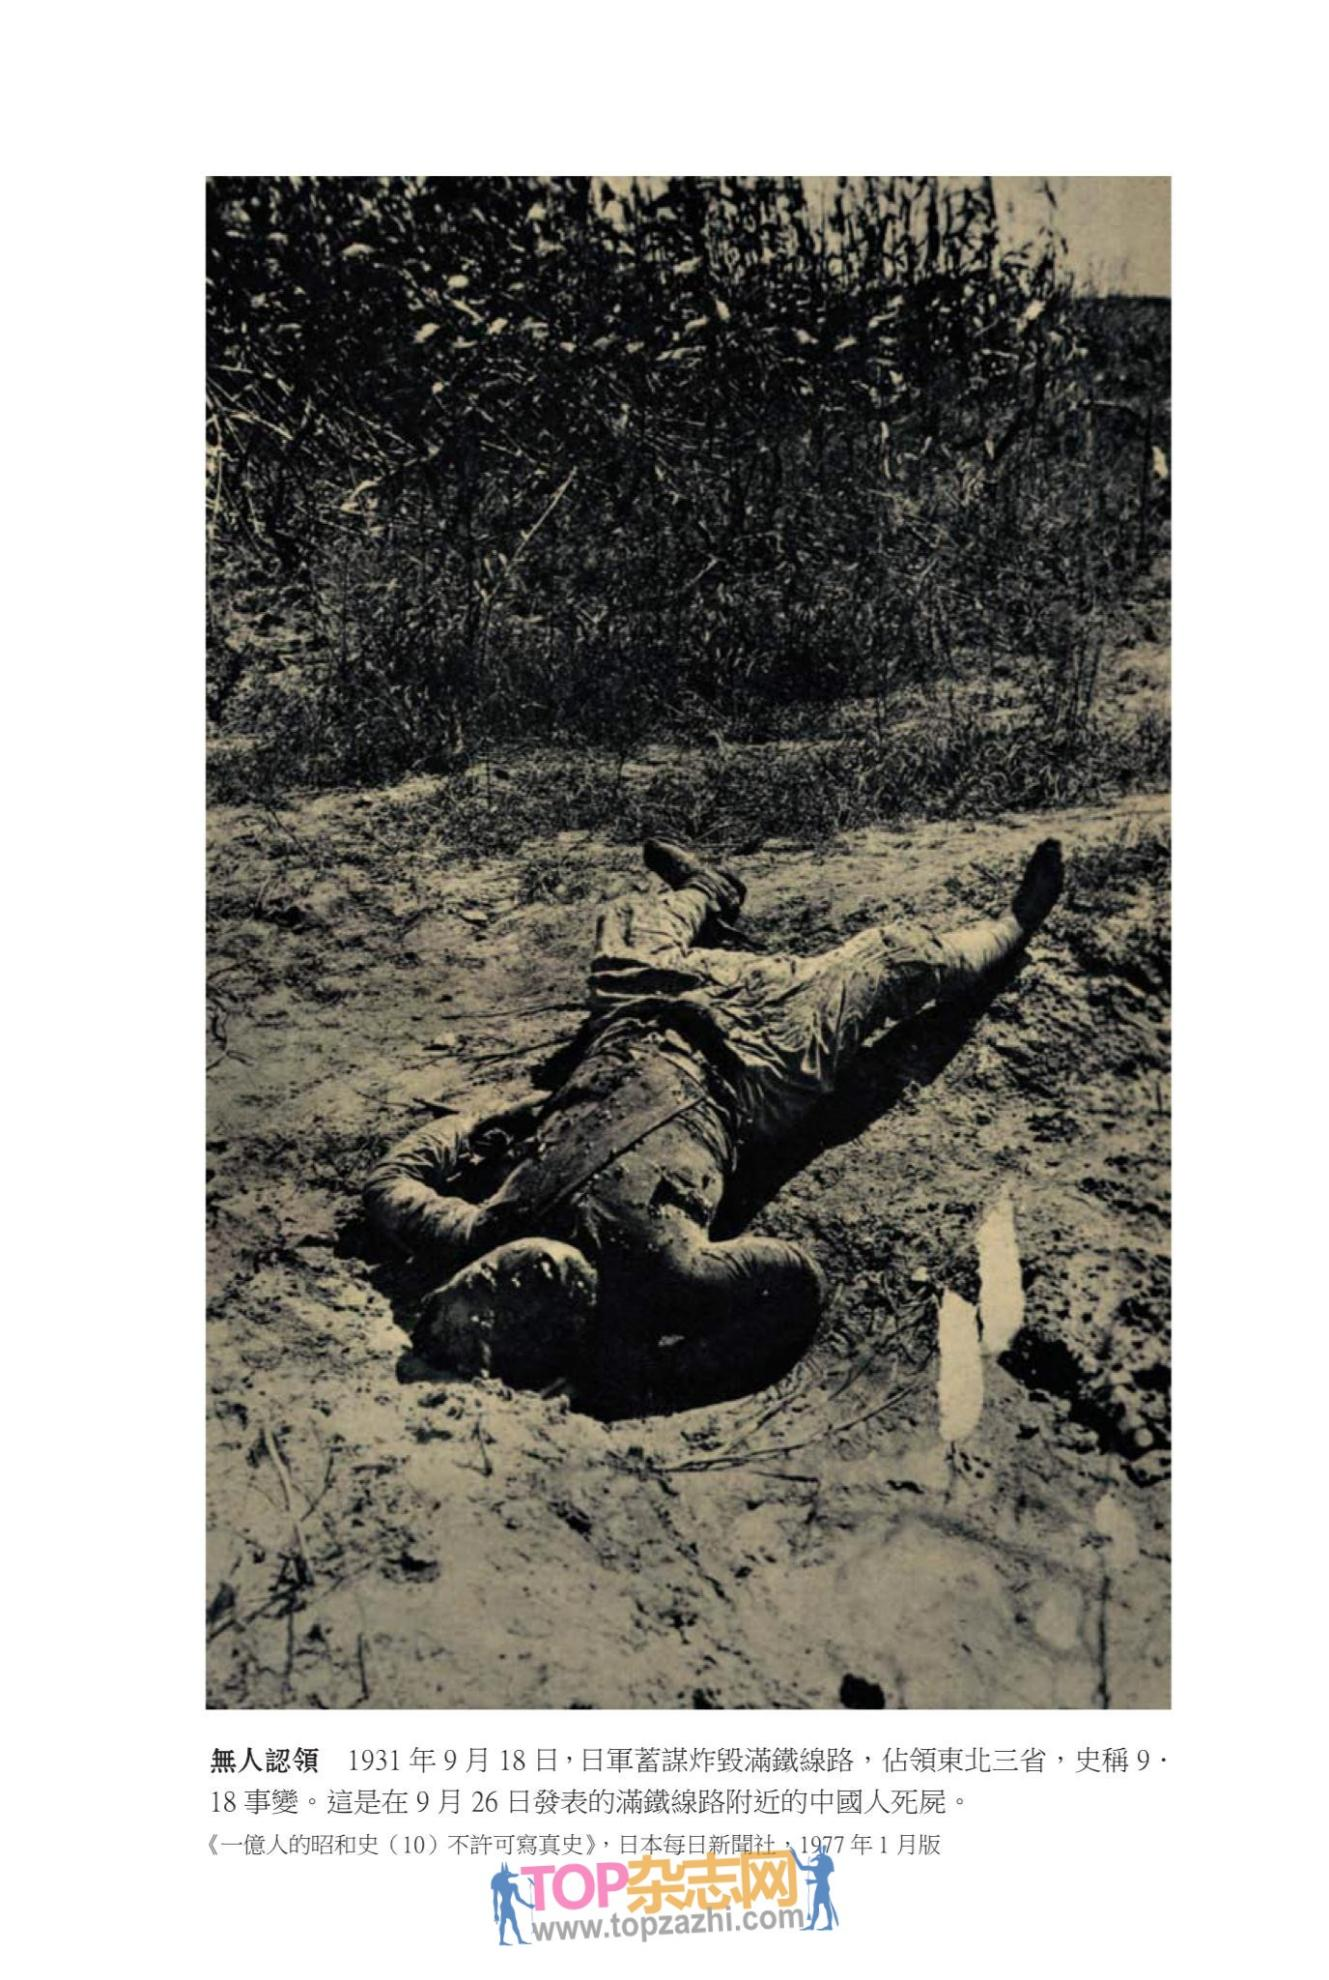
\includegraphics[width=0.7\linewidth]{1}
	\caption{}
	\label{fig:1}
\end{figure}



\chapter{1937年12月13日~1937年12月31日}

\section{1937.12.13}

\subsection{1}

鬆井石根(陸軍大将,日軍華中方面軍最高司令官)

到此為止,我军占領了整個南京。

\subsection{2}

拉貝(John H·D·Rabe·德國·西門子洋行南京代表,南京安全區國際委员會主席)

大清早,空襲再次把我驚醒時,我感到非常失望。炸彈又一次像冰雹般地落了下来。昨天晚上,日軍只攻估了幾座城門,沒有推進到城内。

\chapter{1938年1月1日~1938年2月13日}


\backmatter

\chapter{隐痛(代后记)}
\chapter{致谢}
\chapter{文献来源}

\end{document}